\chapter{Bayesian machine learning}\label{chap13}

\section*{Solutions of Exercises}\label{sec13_1}
\begin{enumerate}[leftmargin=*]

	\item \textbf{Simulation exercise: the Bayesian LASSO continues}

Program the Gibbs sampler for the Bayesian LASSO from scratch, assuming a hierarchical structure for the global shrinkage parameter, where both the shape and rate parameters are set to 1. Perform inference using this sampler in the Bayesian LASSO simulation exercise and compare the results with those obtained using the \textit{monomvn} package.\\

\textbf{Answer}

The following code illustrates how to implement the Gibbs sampler for the Bayesian LASSO. Overall, the results are very similar to those obtained using the \textit{monomvn} package (see Figure~\ref{figLASSOperf}).

\begin{tcolorbox}[enhanced,width=4.67in,center upper,
	fontupper=\large\bfseries,drop shadow southwest,sharp corners]
	\textit{R code. Simulation: The Bayesian LASSO}
	\begin{VF}
		\begin{lstlisting}[language=R]
rm(list = ls()); set.seed(10101)
library(monomvn)
# Parameters
n <- 500  # sample size
k <- 100  # number of predictors
s <- 10   # number of non-zero coefficients
# Generate design matrix
X <- matrix(rnorm(n * k), nrow = n, ncol = k)
# True beta: first s coefficients are non-zero, rest are zero
beta_true <- c(runif(s, -3, 3), rep(0, k - s))
# Generate response with some noise
sigma <- 1
y <- X %*% beta_true + rnorm(n, sd = sigma)
df <- data.frame(X,y)
### Using monomvn ###
library(monomvn)
library(statmod)
# Fit model using Bayesian LASSO
fit <- monomvn::blasso(X, y, T = 5000, verb = 0)
# burn-in removal
burnin <- 1000
beta_samples <- fit$beta[(burnin + 1):5000, ]  # exclude burn-in
intercept_samples <- fit$mu[(burnin + 1):5000] # intercept posterior draws
# Posterior mean of coefficients
beta_post_mean <- colMeans(beta_samples)
# Intercept summary
mean(intercept_samples)
quantile(intercept_samples, c(0.025, 0.975))
# Local shrinkage parameters
colMeans(is.na(fit$tau2i))  # proportion of NA values per coefficient

#### Gibss sampler ####
# Hyperparameters
r0 <- 1; d0 <- 1
# MCMC parameters
mcmc <- 5000; burnin <- 5000
tot <- mcmc + burnin; thin <- 1
# Posterior distributions programming the Gibbs sampling
# Standardized variables
W <- scale(X)
yh <- y - mean(y)
# Gibbs sampling functions
PostBeta <- function(sig2, tau2){
	Bn <- solve(diag(1/tau2) + t(W)%*%W)
	bn <- Bn%*%t(W)%*%yh
	Beta <- MASS::mvrnorm(1, bn, sig2*Bn)
	return(Beta)
}
\end{lstlisting}
	\end{VF}
\end{tcolorbox} 
 
\begin{tcolorbox}[enhanced,width=4.67in,center upper,
	fontupper=\large\bfseries,drop shadow southwest,sharp corners]
	\textit{R code. Simulation: The Bayesian LASSO}
	\begin{VF}
		\begin{lstlisting}[language=R]
PostSig2 <- function(Beta, tau2){
	an <- n - 1 + k
	dn <- t(yh - W%*%Beta)%*%(yh - W%*%Beta) + t(Beta)%*%diag(1/tau2)%*%Beta
	sig2 <- invgamma::rinvgamma(1, shape = an/2, rate = dn/2)
	return(sig2)
}
PostTau2 <- function(sig2, Beta, lambda, p){
	mukn <- (lambda^2*sig2/Beta[p]^2)^0.5
	lambdan <- lambda^2
	tauk2k <- rinvgauss(1, mean = mukn, shape = lambdan)
	return(tauk2k)
}
PostLambda2 <- function(tau2){
	sh <- k + r0
	rat <- 0.5 * sum(tau2) + d0
	lambda2 <- rgamma(1, shape = sh, rate = rat)
	return(lambda2^0.5)
}
PostBeta0 <- function(sig2){
	beta0 <- rnorm(1, mean = mean(y), sd = (sig2/n)^0.5)
	return(beta0)
}
PostBetas <- matrix(0, mcmc+burnin, k)
PostSigma2 <- rep(0, mcmc+burnin)
PostTaus2 <- matrix(0, mcmc+burnin, k)
PostLambda <- rep(0, mcmc+burnin)
PostBetas0 <- rep(0, mcmc+burnin)
Beta <- rep(0, k); tau2 <- rep(1, k); lambda <- 1
# create progress bar in case that you want to see iterations progress
pb <- winProgressBar(title = "progress bar", min = 0, max = tot, width = 300)
for(s in 1:tot){
	sig2 <- PostSig2(Beta = Beta, tau2 = tau2)
	PostSigma2[s] <- sig2
	Beta <- PostBeta(sig2 = sig2, tau2 = tau2)
	PostBetas[s,] <- Beta
	tau2 <- sapply(1:k, function(i){PostTau2(sig2 = sig2, Beta = Beta, lambda = lambda, p = i)})
	PostTaus2[s,] <- tau2
	lambda <- PostLambda2(tau2 = tau2)
	PostLambda[s] <- lambda
	beta0 <- PostBeta0(sig2 = sig2)
	PostBetas0[s] <- beta0
	setWinProgressBar(pb, s, title=paste( round(s/tot*100, 0), "% done"))
}
close(pb)
keep <- seq((burnin+1), tot, thin)
PosteriorBetas <- PostBetas[keep,]
summary(coda::mcmc(PosteriorBetas))
PosteriorBeta0 <- PostBetas0[keep]
summary(coda::mcmc(PosteriorBeta0))
PosteriorSigma2 <- PostSigma2[keep]
summary(coda::mcmc(PosteriorSigma2))
PosteriorTau2s <- PostTaus2[keep,]
summary(coda::mcmc(PosteriorTau2s))
PosteriorLambda <- PostLambda[keep]
summary(coda::mcmc(PosteriorLambda))
\end{lstlisting}
	\end{VF}
\end{tcolorbox} 

\begin{tcolorbox}[enhanced,width=4.67in,center upper,
	fontupper=\large\bfseries,drop shadow southwest,sharp corners]
	\textit{R code. Simulation: The Bayesian LASSO}
	\begin{VF}
		\begin{lstlisting}[language=R]
# Posterior mean of coefficients
beta_post_meanNew <- colMeans(PosteriorBetas)
# Plot true vs estimated betas
plot(beta_true, beta_post_mean, pch = 19, col = "steelblue",
xlab = "True beta", ylab = "Posterior mean of beta",
main = "Bayesian LASSO (blasso): Shrinkage Effect")
abline(0, 1, col = "red", lty = 2)
# Add another set of posterior means
points(beta_true, beta_post_meanNew, pch = 17, col = "darkorange")
# Add legend
legend("topleft", legend = c("blasso", "Our Gibbs"), 
col = c("steelblue", "darkorange"), 
pch = c(19, 17), bty = "n")
		\end{lstlisting}
	\end{VF}
\end{tcolorbox} 

\begin{figure}[!h]
	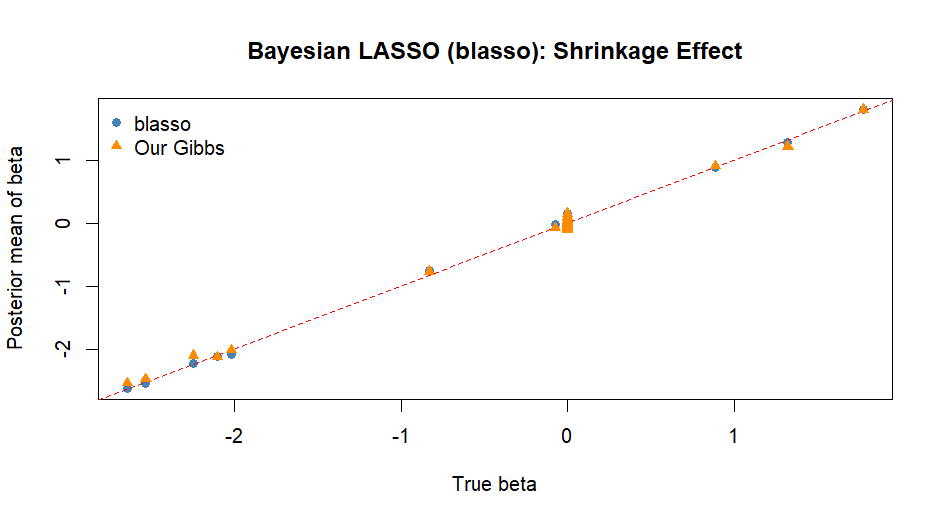
\includegraphics[width=340pt, height=200pt]{Chapters/chapter13/figures/figLASSOperf.png}
	\caption[List of figure caption goes here]{Comparison of LASSO performance: Package vs Gibbs from scratch.}\label{figLASSOperf}
\end{figure}

\item \cite{jetter2022postcold} employ  stochastic search variable selection (SSVS) to identify the main drivers of civil conflict in the post-Cold War era, considering a set of 35 potential determinants across 175 countries worldwide. We use a subset of their dataset provided in \textit{Conflict.xlsx}, where the dependent variable is \textit{conflictcw}, a binary indicator of civil conflict. Perform SSVS using the \textit{BoomSpikeSlab} package, specifically the \textit{lm.spike} function, to identify the best subset of models.\\

\textbf{Answer}

The following code illustrates how to implement SSVS in this application, based on \cite{jetter2022postcold}, using 15,000 iterations and the default settings for the hyperparameters. We find that infant mortality rate, population, peace, and political rights are the most relevant drivers of the incidence of civil conflict. \textit{Peace} exhibits a negative 95\% credible interval, while the other variables have positive credible intervals. The model with the highest posterior probability (30\%) includes the first three regressors.

\begin{tcolorbox}[enhanced,width=4.67in,center upper,
	fontupper=\large\bfseries,drop shadow southwest,sharp corners]
	\textit{R code. Application: Drivers of civil conflict in the post-Cold War era using a linear model}
	\begin{VF}
		\begin{lstlisting}[language=R]
rm(list = ls())
set.seed(010101)
Data <- read.csv("https://raw.githubusercontent.com/BEsmarter-consultancy/BSTApp/refs/heads/master/DataApp/Conflict.csv", sep = ",", header = TRUE, quote = "")

# Scale regressors
W <- as.matrix(scale(Data[, -c(1, 2)]))
niter <- 15000
y <- unlist(Data[, 2])

# Linear model
SSBoomLinear <- lm.spike(y ~ W, niter = niter)
Models <- SSBoomLinear$beta != 0
PIP <- colMeans(SSBoomLinear$beta != 0)
# Convert the logical matrix to a data frame and then to a tibble
df <- as.data.frame(Models); df_tbl <- as_tibble(df)
# Count identical rows
row_counts <- df_tbl %>% count(across(everything()), name = "frequency") %>% arrange(desc(frequency))
colnames(W)
# Get indices of best model
for(l in 1:5) {
	print(which(row_counts[l,] == 1))
	print(row_counts[l, dim(row_counts)[2]]/niter)
}
# Coefficients
SummarySS <- summary(coda::mcmc(SSBoomLinear$beta))
SummarySS
\end{lstlisting}
	\end{VF}
\end{tcolorbox} 


\item \cite{tuchler2008bayesian} proposes an SSVS approach for binary response models. Use the dataset \textit{Conflict.xlsx}, where the dependent variable is \textit{conflictcw}, to perform SSVS using the \textit{BoomSpikeSlab} package, specifically the \texttt{logit.spike} function, in order to identify the best subset of models. Compare the results with those obtained in Exercise 2.\\

\textbf{Answer}

The following code illustrates how to implement SSVS in this application, based on \cite{jetter2022postcold}, using 15,000 iterations and the default settings for the hyperparameters with a logit model. 

We find that the results using a logit model are very similar to those obtained with a linear model. Once again, infant mortality rate, population, peace, and political rights emerge as the most relevant drivers of the incidence of civil conflict. \textit{Peace} exhibits a negative 95\% credible interval, while the other variables have positive credible intervals. In this case, the model with the highest posterior probability (35\%) includes infant mortality rate and peace. However, the model with the second-highest posterior probability (17\%) includes the first three drivers.

\begin{tcolorbox}[enhanced,width=4.67in,center upper,
	fontupper=\large\bfseries,drop shadow southwest,sharp corners]
	\textit{R code. Application: Drivers of civil conflict in the post-Cold War era using a logit model}
	\begin{VF}
		\begin{lstlisting}[language=R]
rm(list = ls())
set.seed(010101)
Data <- read.csv("https://raw.githubusercontent.com/BEsmarter-consultancy/BSTApp/refs/heads/master/DataApp/Conflict.csv", sep = ",", header = TRUE, quote = "")

# Scale regressors
W <- as.matrix(scale(Data[, -c(1, 2)]))
niter <- 15000
y <- unlist(Data[, 2])

# Logit model
SSBoomLogit <- logit.spike(y ~ W, niter = niter)
ModelsLogit <- SSBoomLogit$beta != 0
PIPLogit <- colMeans(SSBoomLogit$beta != 0)
# Convert the logical matrix to a data frame and then to a tibble
df <- as.data.frame(ModelsLogit); df_tbl <- as_tibble(df)
# Count identical rows
row_counts <- df_tbl %>% count(across(everything()), name = "frequency") %>% arrange(desc(frequency))
colnames(W)
# Get indices of best model
for(l in 1:5) {
	print(which(row_counts[l,] == 1))
	print(row_counts[l, dim(row_counts)[2]]/niter)
}
# Coefficients
SummarySSlogit <- summary(coda::mcmc(SSBoomLogit$beta))
SummarySSlogit
		\end{lstlisting}
	\end{VF}
\end{tcolorbox} 

\item \textbf{Example: Simulation exercise $K > N$}

Use the simulation setting from the Bayesian LASSO and SSVS examples, but now assume there are 600 features. This setup implies that the number of features exceeds the sample size. In such a scenario, there is no unique solution to the least squares estimator because the determinant of $\mathbf{W}^{\top} \mathbf{W}$ is zero. This means the matrix is not invertible, and consequently, standard inference procedures based on the least squares estimator cannot be applied. On the other hand, Bayesian inference in this setup is well-defined because the prior helps regularize the problem, which is a key motivation for these methods.\\

\textbf{Answer}

The following code shows how to perform this exercise using the \textit{bayesreg} and \textit{BoomSpikeSlab} packages. We observe that both the Bayesian LASSO and SSVS perform well (see Figure~\ref{figKlargerN}) and allow for valid inference.

\begin{tcolorbox}[enhanced,width=4.67in,center upper,
	fontupper=\large\bfseries,drop shadow southwest,sharp corners]
	\textit{R code. Simulation: Performance of the Bayesian LASSO and SSVS when $K > N$}
	\begin{VF}
		\begin{lstlisting}[language=R]
rm(list = ls()); set.seed(10101)
library(BoomSpikeSlab)
library(dplyr)
library(tibble)
library(bayesreg)
# Parameters
n <- 500  # sample size
k <- 600  # number of predictors
s <- 10   # number of non-zero coefficients
# Generate design matrix
X <- matrix(rnorm(n * k), nrow = n, ncol = k)
# True beta: first s coefficients are non-zero, rest are zero
beta_true <- c(runif(s, -3, 3), rep(0, k - s))
# Generate response with some noise
sigma <- 1
y <- X %*% beta_true + rnorm(n, sd = sigma)
df <- data.frame(X,y)
### Using BoomSpikeSlab ###
#Scale regressors
W <- scale(X); yh <- y - mean(y)
niter <- 5000
######Estimate model########
# Least squared
Reg <- lm(y ~ X)
summary(Reg)
## BLASSO ##
# Fit the model
fit <- bayesreg::bayesreg(y ~ X, data = df, model = "gaussian", prior = "lasso", 
n.samples = niter, burnin = 1000)
# Check summary
summary(fit)
# Extract posterior means of beta
beta_post_meanLASSO <- rowMeans(fit$beta)

## SSVS ##
SSBoomNew <- lm.spike(yh ~ W - 1, niter = niter)
# Coefficients
SummarySS <- summary(coda::mcmc(SSBoomNew$beta))
# Extract posterior means of beta
beta_post_meanSSVS <- SummarySS$statistics[, 1]

# Compare true vs estimated
plot(beta_true, beta_post_meanLASSO, pch = 19, col = "steelblue",
xlab = "True beta", ylab = "Posterior mean of beta",
main = "Bayesian LASSO and SSVS")
abline(0, 1, col = "red", lty = 2)
# Add another set of posterior means
points(beta_true, beta_post_meanSSVS, pch = 17, col = "darkorange")
# Add legend
legend("topleft", legend = c("BLASSO", "SSVS"), 
col = c("steelblue", "darkorange"), 
pch = c(19, 17), bty = "n")
\end{lstlisting}
	\end{VF}
\end{tcolorbox} 

\begin{figure}[!h]
	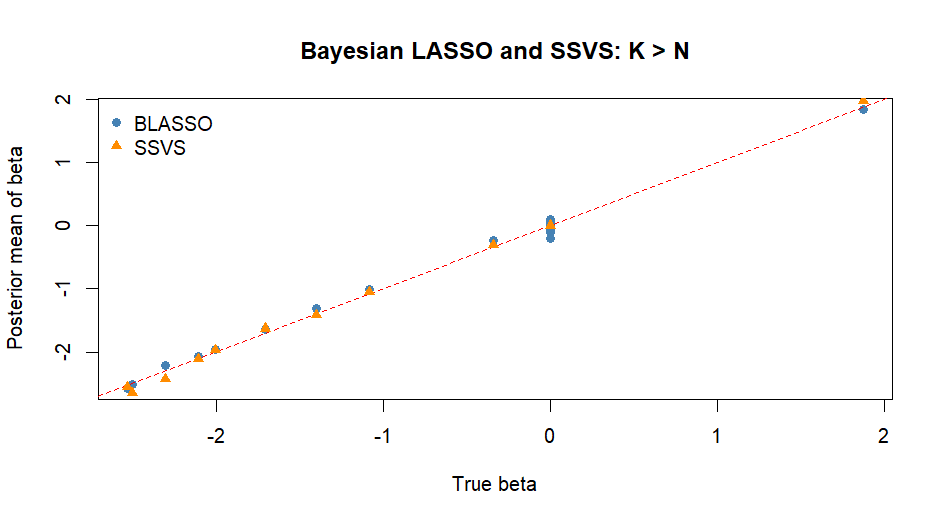
\includegraphics[width=340pt, height=200pt]{Chapters/chapter13/figures/KlargerN.png}
	\caption[List of figure caption goes here]{Performance of the Bayesian LASSO and SSVS: $K > N$.}\label{figKlargerN}
\end{figure}

\item \textbf{Simulation exercise: the BART model continues} 

Compute Friedman’s partial dependence functions \cite{friedman2001greedy} for all variables in the BART model simulation example, and plot the posterior mean along with the 95\% credible intervals.

\textbf{Answer}

The following code illustrates how to compute the posterior distribution of Friedman’s partial dependence functions. Figures \ref{figPartial1} and \ref{figPartial10} display the results for variables 1 and 10. From the simulation setup, we know that variable 1 is relevant, whereas variable 10 is irrelevant. This is reflected in the partial dependence functions: the function for variable 10 is flat, indicating no effect, while the function for variable 1 shows a positive relationship with the outcome variable.


\begin{tcolorbox}[enhanced,width=4.67in,center upper,
	fontupper=\large\bfseries,drop shadow southwest,sharp corners]
	\textit{R code. Simulation: Partial dependence functions from BART models}
	\begin{VF}
		\begin{lstlisting}[language=R]
rm(list = ls()); set.seed(10101)
library(BART); library(ggplot2); library(dplyr); library(tidyr)
N <- 500; K <- 10
# Simulate the dataset
MeanFunct <- function(x){
	f <- 10*sin(pi*x[,1]*x[,2]) + 20*(x[,3]-.5)^2+10*x[,4]+5*x[,5]
	return(f)
}
sig2 <- 1
e <- rnorm(N, 0, sig2^0.5)
X <- matrix(runif(N*K),N,K)
y <- MeanFunct(X[,1:5]) + e
# Hyperparameters
alpha <- 0.95; beta <- 2; k <- 2
v <- 3; q <- 0.9; J <- 200
# MCMC parameters
MCMCiter <- 1000; burnin <- 100; thinning <- 1
# Partial dependence function
BARTfit <- wbart(x.train = X, y.train = y, base = alpha,
power = beta, k = k, sigdf = v, sigquant = q, ntree = J,
ndpost = MCMCiter, nskip = burnin, keepevery = thinning)
k <- 1; L <- 20
x <- seq(min(X[, k]), max(X[, k]), length.out = L)
X.test <- X
X.test[,k] <- x[1]
for(j in 2:L){
	X.k <- X
	X.k[,k] <- x[j]
	X.test <- rbind(X.test, X.k)
} 
pred <- predict(BARTfit, X.test)
partial <- matrix(nrow = MCMCiter, ncol = L)
for(j in 1:L) {
	h <- (j - 1) * N + 1:N
	partial[, j] <- apply(pred[, h], 1, mean)
}
partial_df <- as.data.frame(partial)
partial_df$draw <- 1:nrow(partial_df)
long_df <- pivot_longer(partial_df, cols = -draw, names_to = "x", values_to = "value")
long_df$x <- as.numeric(gsub("V", "", long_df$x))
summary_df <- long_df %>% group_by(x) %>%
summarise(mean = mean(value), lower = quantile(value, 0.025), upper = quantile(value, 0.975)
)
ggplot(summary_df, aes(x = x, y = mean)) + geom_line(color = "blue") + geom_ribbon(aes(ymin = lower, ymax = upper), fill = "lightblue", alpha = 0.4) + labs(x = "Grid point", y = "Partial effect", title = "Partial Dependence Function with 95% Intervals") + theme_minimal()
\end{lstlisting}
	\end{VF}
\end{tcolorbox} 

\begin{figure}[!h]
	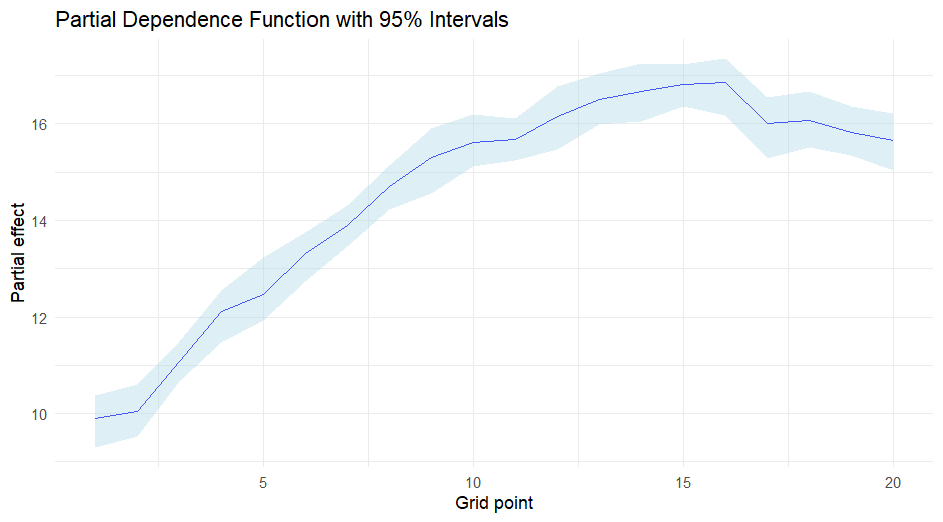
\includegraphics[width=340pt, height=200pt]{Chapters/chapter13/figures/Partial1.png}
	\caption[List of figure caption goes here]{Partial dependence function: Variable 1.}\label{figPartial1}
\end{figure}

\begin{figure}[!h]
	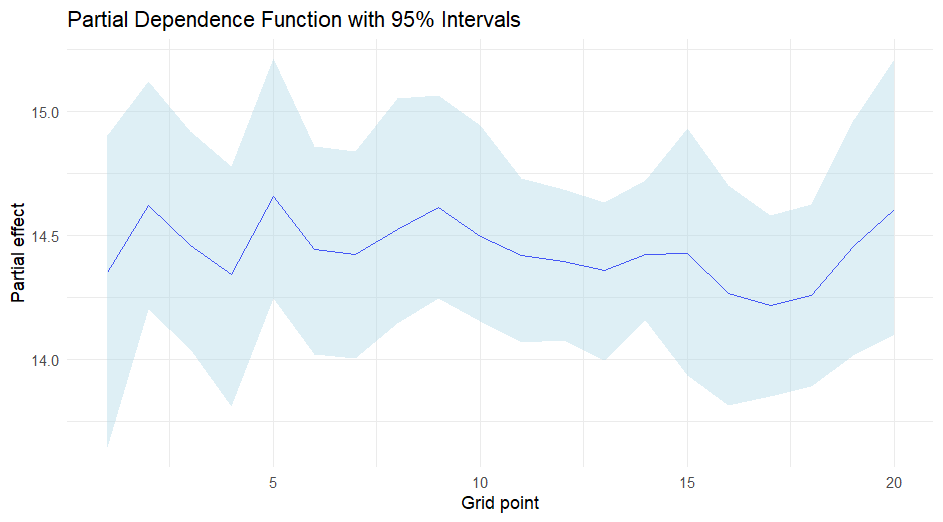
\includegraphics[width=340pt, height=200pt]{Chapters/chapter13/figures/Partial10.png}
	\caption[List of figure caption goes here]{Partial dependence function: Variable 10.}\label{figPartial10}
\end{figure}

\item \textbf{Simulation exercise: The Gaussian Process simulation continues}

	Simulate the process
\[
f_i = \sin(2\pi x_{i1}) + \cos(2\pi x_{i2}) + \sin(x_{i1} x_{i2}) + \mu_i,
\]
where \( \mu_i \overset{\text{i.i.d.}}{\sim} {N}(0, 0.1^2) \), \( x_{ik} \sim {U}(0,1) \) for \( k = 1, 2 \), and the sample size is 500. 

Define a grid of 20 evenly spaced values between 0 and 1 for each covariate \( x_{ik} \), and use this grid to perform prediction.

Estimate the hyperparameters of the Gaussian Process by maximizing the log marginal likelihood. Then, use the \textit{km} function from the \textit{DiceKriging} package to fit the Gaussian Process, fixing the noise variance at the value that maximizes the log marginal likelihood.

Finally, use the fitted model to predict the outputs on the grid points, and produce a 3D plot showing the predicted surface along with the training data points.

\textbf{Answer} 

We use the Cholesky decomposition to optimize time calculating the inverse of the covariance matrix. In particular, let \( \mathbf{K} \in \mathbb{R}^{N \times N} \) be a symmetric positive definite matrix. Then, it admits a Cholesky decomposition:
	
	\[
	\mathbf{K} = \mathbf{L} \mathbf{L}^\top,
	\]
	
	where \( \mathbf{L} \) is a lower triangular matrix with positive diagonal entries.
	
	The determinant of \( \mathbf{K} \) can be computed using the Cholesky factor:
	
	\[
	\det(\mathbf{K}) = \det(\mathbf{L} \mathbf{L}^\top) = \det(\mathbf{L})^2.
	\]
	
	Since \( \mathbf{L} \) is lower triangular, its determinant is the product of its diagonal elements:
	
	\[
	\det(\mathbf{K}) = \left( \prod_{i=1}^N L_{ii} \right)^2.
	\]
	
	Equivalently, the log-determinant is:
	
	\[
	\log |\mathbf{K}| = 2 \sum_{i=1}^N \log L_{ii}.
	\]
	
	The inverse of \( \mathbf{K} \) can also be computed using the Cholesky factor:
	
	\[
	\mathbf{K}^{-1} = (\mathbf{L} \mathbf{L}^\top)^{-1} = (\mathbf{L}^\top)^{-1} \mathbf{L}^{-1}.
	\]
	
	This is useful computationally because triangular systems can be solved efficiently via forward and backward substitution:
	
	\begin{enumerate}
		\item Solve \( \mathbf{L} \mathbf{z} = \mathbf{b} \) for \( \mathbf{z} \) (forward solve),
		\item Solve \( \mathbf{L}^\top \mathbf{x} = \mathbf{z} \) for \( \mathbf{x} \) (backward solve),
	\end{enumerate}
	
	then,  \( \mathbf{x} = (\mathbf{L}^\top)^{-1} \mathbf{z} = (\mathbf{L}^\top)^{-1} \mathbf{L}^{-1}  \mathbf{b} = (\mathbf{L}\mathbf{L}^\top)^{-1} \mathbf{b} = \mathbf{K}^{-1}  \mathbf{b} \).
	Thus, we avoid computing the matrix inverse, which requires \( O(N^3) \) operations. Instead, it is more efficient and numerically stable to solve triangular systems of equations, which arise naturally from the Cholesky decomposition.
	
	The following code shows how to perform this exercise, and Figure \ref{GPsim3D} displays the 3D plot.
	
\begin{tcolorbox}[enhanced,width=4.67in,center upper,
	fontupper=\large\bfseries,drop shadow southwest,sharp corners]
	\textit{R code. Simulation: $f_i=\sin(2\pi x_{i1}) + \cos(2\pi x_{i2}) + \sin(x_{i1} x_{i2}) + \mu_i$ and Gaussian process}
	\begin{VF}
		\begin{lstlisting}[language=R]
rm(list = ls()); set.seed(10101)
library(fields); library(DiceKriging); library(ggplot2)
# Simulate training data
n_train <- 500
x1 <- runif(n_train); x2 <- runif(n_train)
X_train <- data.frame(x1 = x1, x2 = x2)
sig <- 0.1; u <- rnorm(n_train, mean = 0, sd = sig)
# True function without noise
f_train <- sin(2 * pi * X_train$x1) + cos(2 * pi * X_train$x2) + sin(X_train$x1 * X_train$x2)
y_train <- scale(f_train + u)
# Empirical Bayes: Optimize the log marginal likelihood
log_marginal_likelihood <- function(par, X, y) {
	sigma2_f <- par[1]; l2 <- par[2]; sigma2_n <- par[3]; n <- nrow(X)
	# Ensure parameters are positive
	if (sigma2_f <= 0 | l2 <= 0 | sigma2_n <= 0) return(Inf)
	# Squared exponential kernel
	dists <- rdist(X)
	K <- sigma2_f * exp(-0.5 * (dists^2) / l2)
	# Add noise variance + jitter for numerical stability
	K <- K + (sigma2_n + 1e-8) * diag(n)
	# Cholesky decomposition
	L <- tryCatch(chol(K), error = function(e) return(NULL))
	if (is.null(L)) return(Inf)
	alpha <- backsolve(t(L), forwardsolve(L, y)) #--> K^{-1}y
	log_det_K <- 2 * sum(log(diag(L)))
	lml <- -0.5 * t(y) %*% alpha - 0.5 * log_det_K - 0.5 * n * log(2 * pi)
	return(-as.numeric(lml))  # Negative log-marginal likelihood
}
par0 <- rep(1, 3)
ResOpt <- optim(par = par0, fn = log_marginal_likelihood, method = "L-BFGS-B", lower = c(1e-5, 1e-5), X = X_train, y = y_train)
theta_hat <- ResOpt$par
sigma2_f_hat <- theta_hat[1]; l2_hat <- theta_hat[2]; sigma2_n_hat <- theta_hat[3]
# Grid for prediction 
grid_points <- 20
x1_seq <- seq(0, 1, length.out = grid_points)
x2_seq <- seq(0, 1, length.out = grid_points)
X_new <- expand.grid(x1 = x1_seq, x2 = x2_seq)
# Fit Gaussian Process
fit_km <- km(design = X_train, response = y_train, covtype = "gauss", noise.var = rep(sigma2_n_hat, n_train))
# Predict GP surface
pred <- predict(fit_km, newdata = X_new, type = "UK")
z_pred <- matrix(pred$mean, nrow = grid_points, ncol = grid_points)
# Plot
persp3d(x = x1_seq, y = x2_seq, z = z_pred, col = "lightblue", alpha = 0.7, xlab = "x1", ylab = "x2", zlab = "GP Mean")
points3d(x = X_train$x1, y = X_train$x2, z = y_train, col = "red", size = 8)
\end{lstlisting}
	\end{VF}
\end{tcolorbox}

\begin{figure}[!h]
	\centering
	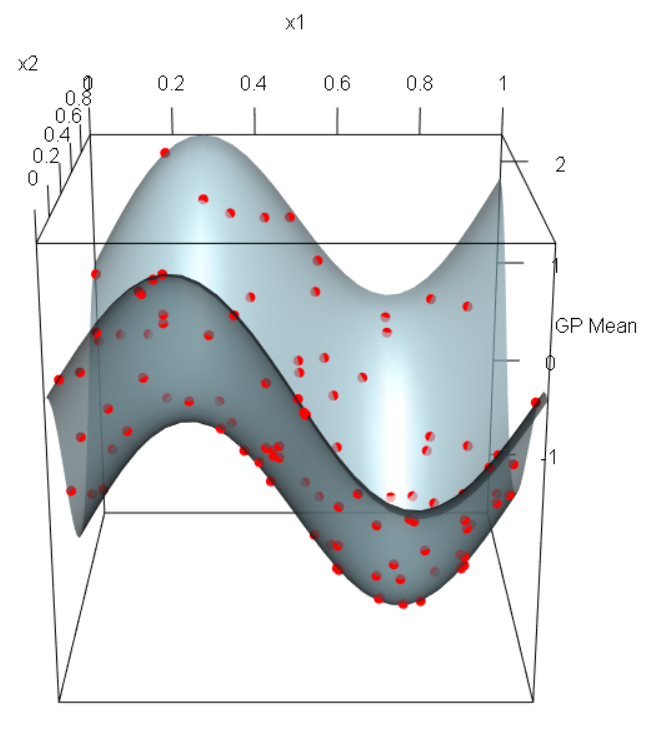
\includegraphics[width=340pt, height=200pt]{Chapters/chapter13/figures/GPsim3D.png}
	\caption{Simulation: $f_i=\sin(2\pi x_{i1}) + \cos(2\pi x_{i2}) + \sin(x_{i1} x_{i2}) + \mu_i$ and Gaussian process}
	\label{GPsim3D}
\end{figure} 

	
	
	

\end{enumerate}